% !TEX root = ../thesis.tex
\chapter{Context-Aware Data Mashups: Concepts, Goals and Requirements}
\label{capitolo3}
\thispagestyle{empty}

\section{Concepts}
\subsection{Introducing CAMUS}
Context-Aware Data MashUpS (CAMUS)\cite{camus} is a project that aims to dynamically generate mobile applications, based on a framework capable of performing seamless data integration of resources obtained from multiple heterogeneous sources, and then apply context-based filtering to this data. The result of this process is an answer that is context-aware; in other words, it takes into account the particular details of the user requesting this information. Moreover, this answer integrates the different responses received from the various sources, whether they are online web services, or locally stored data.\\\\
The CAMUS project is split into multiple components, each having its own purpose and functionality. Moreover, there are multiple human agents involved in operating the system, each of them with their own roles and responsibilities which we will shortly explain. The main components on the CAMUS system are the end-user interface, the context dimension tree, the resource schema, and finally the backend server. On the other hand, the human agents who are involved in this system are the end user, the domain expert, and the system administrator.\\\\\\
\begin{figure}[h]
\includegraphics[width=\textwidth]{camus}
\caption{CAMUS Flow}
\end{figure}
\noindent Figure 3.1 shows the basic operational flow of the CAMUS system. There are two main stages in the operational flow: the initial setup, and the runtime operation. The initial setup starts with the end-user providing their context parameters to the domain expert. The domain expert perform pruning operations on the CDT so that it reflects the user's context. This CDT is initially constructed by the system administrator, and the domain expert can also provide input to make sure that it is able to accurately represent the user's context. The system administrator also constructs the resource schema, which is a representation of the various relevant interest topics.\\\\
Once the mapping between the CDT and the resource schema is done, the system is ready to be put into use, and the end-user can install the application on their device, which moves us to the runtime stage. This is the stage that is most visible to the end-user; the user starts sending a query using the mobile application, and this query is forwarded to the middleware. At this point, the query is still context-agnostic. The middleware takes care of enriching the query with the context details which were previously supplied (using the CDT), and the enriched query is then sent to the backend server. The backend server queries the various web services, integrating their responses in a format that matches the format specified in the resource schema. This final response is forwarded to the middleware, which in turn forwards it to the mobile application so that it can be displayed to the end-user.\\\\
In what follows, we elaborate on each individual component, and we make use of the previously mentioned travel agent example to better illustrate one of the possible use cases.
\subsubsection{The End-User Application}
The end-user interface represents the mobile application installed on the mobile devices of the users. This mobile application is used as a two-way portal that both displays relevant information that users ask for, as well as takes input from the users to further improve the user experience. During the initial setup phase, the end-user (the tourist in our example) provides as many details about their needs and preferences. These details will be used to describe the ``context'' of the user, along with other parameters that can be collected real-time while they use the application. The travel agent takes the information provided by the tourist, and using a web interface, inputs this information into the system.
\subsubsection{The Context-Dimension Tree (CDT)}
The web interface used by the travel agent is generated based on the context dimension tree. The system administrator initially constructs the tree, and the web interface is the mean through which the domain expert can input the values provided by the end-user. This tree is a representation of the various parameters that are part of a user's context for a given topic. In our example, a user's favorite cuisines, their allergies, and their ambience preference (indoors vs. outdoors) are some of factors that constitute the CDT for the ``Restaurants'' topic. The context, now represented by the CDT, is incorportated into the queries, transforming them from a context-agnostic state to a context-aware one.
\subsubsection{The Resource Schema}
The resource schema, also designed by the system administrator, describes the various topics supported by CAMUS for a certain domain; in other words, it includes the attributes associated with a topic. For example, within the tourism domain, the resource schema specifies that the ``Restaurant'' structure is part of the schema, and it includes attributes such as name, address, phone number, cuisines, rating, and so on. A mapping function takes care of matching these attributes with the CDT, which results in context-aware queries.
\subsubsection{The Backend Server}
The final component of the CAMUS framework is the backend server. This component's task is to perform the actual querying of the various web services when required by the middleware. The middleware receives queries from the end-user application or from the domain expert, and performs the mapping between the CDT and the resource schema if needed. Then, the queries are forwarded to the backend server. This server then identifies which web services to query, sends the requests, and parses the responses. This server is also responsible of performing the data integration operations, transforming the heterogeneous output of the various web services into a homogeneous list that is made accessible to the middleware. In what follows, this component will be the main point of focus, and the aim will be to design and provide a working implementation for it.
\newpage
The overall architecture of CAMUS is shown in figure 3.2.
\begin{figure}[h]
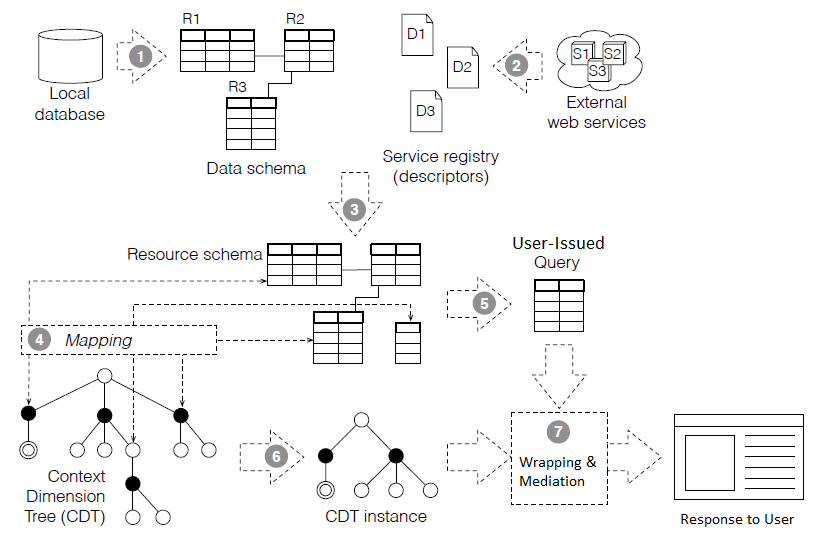
\includegraphics[width=\textwidth]{camarch}
\caption{CAMUS Architecture}
\end{figure}
\subsection{Response format}
In the classical sense, two or more data sets are considered homogenous when they made up of elements that belong to the same type. In other words, all of the elements that make up the data sets share the same structure. The simplest example of a homogenous data set is an array, since generally, all of the elements of an array belong to the same type. Therefore, two integer arrays are homogenous. Conversely, heterogeneous data sets are data sets that contain differently structured elements such as lists and unions, among others. This is the low-level definition of homogeneity and heterogeneity.\\\\
In data integration, two datasets are considered homogenous if they are structured according to the same data model. Naturally, different online services have their own structures for the objects that they return when they receive requests. This is even true for different services that operate in the same domain. For instance, two APIs specializing in food and restaurants reply differently, even if we call a simple search API that returns a list of restaurants. Even though conceptually both APIs are returning a list of restaurants, each API returns different attributes, and therefore the Restaurant objects are not identical. It does not stop at that: even the general structure of the reply, the meta information returned along with the restaurants list, and the names of the fields are different. Therefore, our objective here is to establish pair-wise homogeneity between different responses, in accordance with the structures defined in the resource schema.

\section{Goals and Requirements}

\textbf{\textit{Integration:}} Our primary goal in this thesis is to find a way to extract the useful information from the aforementioned heterogeneous replies, therefore ending up with a homogenous structure (in this example, a collection of restaurants), and this collection will have in it all of the restaurants that were included in the various received replies.\\\\
\textbf{\textit{Context Awareness:}} Context awareness should be included in all of the operational phases of our system. Firstly, selecting which web services to query is made context-aware by choosing services that allow filtering, or include information that match with the parameters that make up our context. These parameters are determined on a case-by-case basis, and therefore, so should be the selected services.\\\\
\textbf{\textit{API Suitability:}} Going to a lower level, the data returned by the services can be enriched with the user's context by making sure that the query parameters of the requests that are being sent to the web services represent as accurately as possible the user's context. In order to do so, each individual API that we are querying should be closely examined, and we should make sure that we are on one hand optimizing the values attached to the query, and that we are taking advantage of all of the supported filtering parameters offered by the web service on the other hand.\\\\\
\textbf{\textit{Flexibility:}} The process should also be flexible, in the sense that, thanks to adaptive abstractions, we should have the ability to add more services, and the algorithm should be able to include the results from the new service without making changes to the core of the code. Instead, we would just have to include a description that specifies details about the new service (what parameters it expects, and the structure of its reply).\\\\
\textbf{\textit{Velocity:}} Another primary concern is to reduce the waiting time on the side of the end user: sending numerous requests to multiple web services, receiving the replies, and parsing these replies can take a lot of time. Therefore, we should aim to reduce the number of sent requests if possible. Mobile application users however do not expect long wait times when performing seemingly simple functions such as searching for a place to eat, and therefore we should be able to provide them with results as soon as possible.\\\\
\textbf{\textit{Request Filtering:}} We have to include the context awareness paradigm in our workflow: the results that the user sees on their device should be filtered according to their own context. In some cases, the filtering can be done before sending the request to the web services, by making use of the request parameters that are sent along with the request.\\\\
\textbf{\textit{Response Filtering:}} Further filtering should be done after the services send their replies: we are bound to encounter services that are not as flexible as we need them to be in terms of allowing filtering within the request parameters. In that case, we should examine all of the fields returned by these services, and make sure that context-based filtering is performed also on these responses when needed. Finally, we should also allow the end-user to provide manually additional filters, to account for changes in the context, or simply to give the user more freedom. This would create a truly dynamic, context-aware output that matches the user's needs as accurately as possible.\\\\
\textbf{\textit{User-friendly Interfaces:}} In order to allow users of CAMUS to easily integrate new services, we should provide an intuitive frontend which can be used to describe new services, and associate them with their respective topics. The same applies to filling a user's information in the CDT, especially that this task should be doable by an individual who does not possess any programming or technical knowledge. Moreover, the system should take into account that the information that was provided as input to the CDT might change over time, and therefore, the implementation should be dynamic enough to allow changes to the CDT, and update the output shown to the users accordingly. To do so, the application installed on the end-user's device must allow them to override the previously-defined context parameters so that they reflect better the current context.\\\\
